\RequirePackage{luatex85}
\documentclass{standalone}
\usepackage{tikz}

% Color Definitions
\definecolor{SourceColor}{RGB}{255,255,255}
\definecolor{TargetColor}{RGB}{255,255,255}
\definecolor{TargetChangerColor}{RGB}{255,255,255}
\definecolor{AbsorbingAreaColor}{RGB}{196,78,82}
\definecolor{ObstacleColor}{RGB}{179,179,179}
\definecolor{StairColor}{RGB}{129,114,178}
\definecolor{MeasurementAreaColor}{RGB}{255,255,255}
\definecolor{InformationAreaColor}{RGB}{255,255,255}
\definecolor{AerosolCloudColor}{RGB}{202,156,76}
\definecolor{AgentColor}{RGB}{76,114,202}
\definecolor{AgentIdColor}{RGB}{255,127,0}
\definecolor{ObstacleGreenColor}{RGB}{10,255,10}
\definecolor{ObstacleBlueColor}{RGB}{179, 236, 255}
\definecolor{ObstacleGreenColor}{RGB}{179, 255, 204}

\newcommand{\MeasurementAreaOpacity}{0.549020}
\newcommand{\AerosolCloudOpacity}{0.039216}

\begin{document}
% Change scaling to [x=1mm,y=1mm] if TeX reports "Dimension too large".
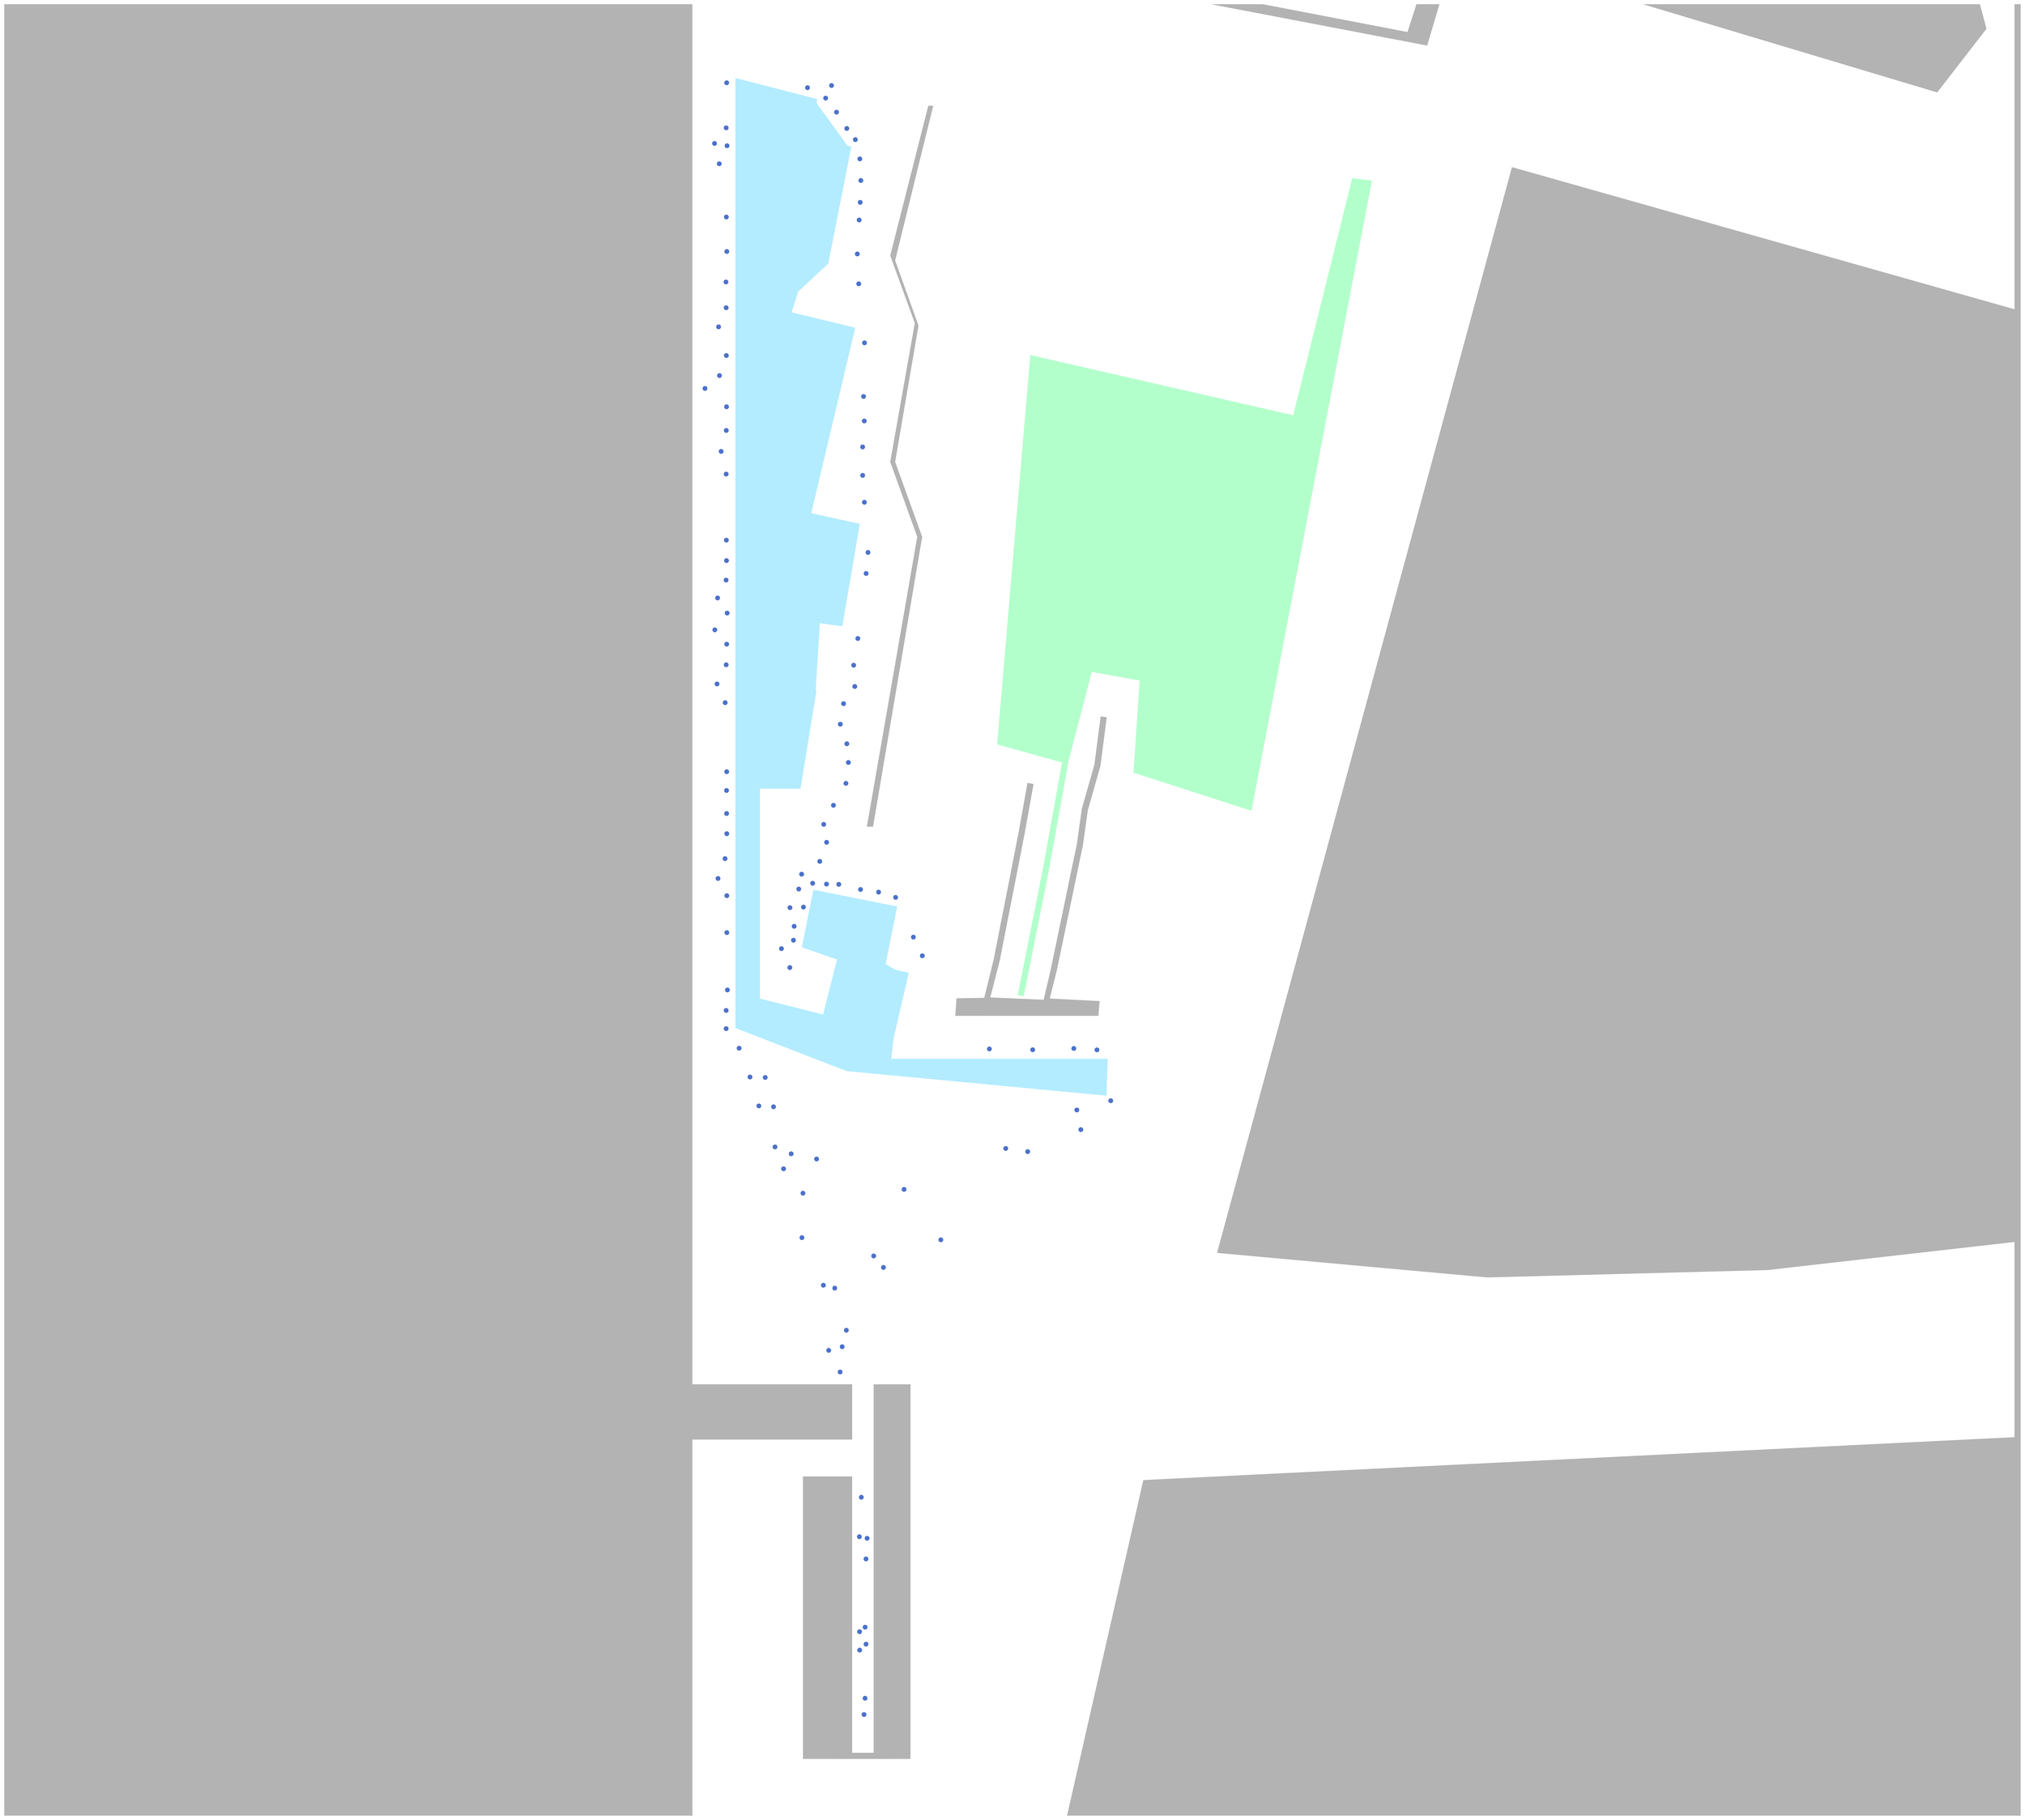
\begin{tikzpicture}
[x=1cm,y=1cm,
trajectory/.style={line width=1},
pedestrian/.style={circle, fill=AgentColor, minimum size=0.390000 cm},
walkdirection/.style={black, line width=1},
selected/.style={draw=magenta, line width=2},
group/.style={},
voronoi/.style={black, line width=1}
]
% Clipping
\clip (0.000000,35.886381) rectangle (164.100000,183.358682);
% Background
\fill[white] (0.000000,0.000000) rectangle (164.100000,215.100000);
% TargetChanger(s)
\coordinate (TargetChanger20) at (57.750000,144.750000); % Centroid: TargetChanger20
\fill[TargetChangerColor] (56.000000,143.000000) to (59.500000,143.000000) to (59.500000,146.500000) to (56.000000,146.500000) to (56.000000,143.000000);
\coordinate (TargetChanger101) at (67.900000,79.000000); % Centroid: TargetChanger101
\fill[TargetChangerColor] (65.699997,77.199997) to (70.099998,77.199997) to (70.099998,80.799995) to (65.699997,80.799995) to (65.699997,77.199997);
\coordinate (TargetChanger23) at (78.650000,99.250000); % Centroid: TargetChanger23
\fill[TargetChangerColor] (77.300003,101.000000) to (80.000000,101.000000) to (80.000000,97.500000) to (77.300003,97.500000) to (77.300003,101.000000);
\coordinate (TargetChanger202) at (70.745128,167.889231); % Centroid: TargetChanger202
\fill[TargetChangerColor] (68.599998,170.100006) to (73.699997,169.300003) to (72.800003,165.699997) to (67.900002,166.399994) to (68.599998,170.100006);
% Source(s)
\coordinate (Source4) at (69.875000,41.750000); % Centroid: Source4
\fill[SourceColor] (69.000000,41.000000) to (70.750000,41.000000) to (70.750000,42.500000) to (69.000000,42.500000) to (69.000000,41.000000);
\coordinate (Source5) at (67.900000,79.000000); % Centroid: Source5
\fill[SourceColor] (65.699997,77.199997) to (70.099998,77.199997) to (70.099998,80.799995) to (65.699997,80.799995) to (65.699997,77.199997);
% Target(s)
\coordinate (Target1000) at (64.181760,102.687914); % Centroid: Target1000
\fill[TargetColor] (66.619545,101.154007) to (61.550381,102.402931) to (61.550381,104.239578) to (66.986870,102.917191) to (66.619545,101.154007);
\coordinate (Target31) at (57.750000,149.150000); % Centroid: Target31
\fill[TargetColor] (56.049999,147.600006) to (56.049999,150.699997) to (59.450001,150.699997) to (59.450001,147.600006) to (56.049999,147.600006);
\coordinate (Target12) at (70.056203,164.708470); % Centroid: Target12
\fill[TargetColor] (72.099998,163.000000) to (67.400002,163.699997) to (67.900002,166.399994) to (72.800003,165.699997) to (72.099998,163.000000);
\coordinate (Target21) at (76.300000,99.275000); % Centroid: Target21
\fill[TargetColor] (75.300003,101.000000) to (77.300003,101.000000) to (77.300003,97.550003) to (75.300003,97.550003) to (75.300003,101.000000);
\coordinate (Target500) at (66.000000,65.000000); % Centroid: Target500
\fill[TargetColor] (65.000000,63.500000) to (67.000000,63.500000) to (67.000000,66.500000) to (65.000000,66.500000) to (65.000000,63.500000);
\coordinate (Target11) at (69.875000,43.000000); % Centroid: Target11
\fill[TargetColor] (69.000000,42.500000) to (70.750000,42.500000) to (70.750000,43.500000) to (69.000000,43.500000) to (69.000000,42.500000);
\coordinate (Target999) at (69.750000,43.000000); % Centroid: Target999
\fill[TargetColor] (69.000000,42.500000) to (70.500000,42.500000) to (70.500000,43.500000) to (69.000000,43.500000) to (69.000000,42.500000);
% AbsorbingArea(s)
% Obstacle(s)
\coordinate (Obstacle10) at (94.483203,194.457168); % Centroid: Obstacle10
\fill[ObstacleColor] (63.000000,190.100006) to (115.800003,180.000000) to (122.500000,202.600006) to (123.800003,214.600006) to (122.699997,214.600006) to (121.099998,202.600006) to (114.199997,181.100006) to (64.300003,190.699997) to (65.099998,214.600006) to (63.500000,214.600006) to (63.000000,190.100006);
\coordinate (Obstacle11) at (144.373315,195.509796); % Centroid: Obstacle11
\fill[ObstacleColor] (134.199997,214.600006) to (127.022583,185.265976) to (157.311188,176.183228) to (161.319824,181.369537) to (157.150406,196.872665) to (151.535873,214.600006) to (134.199997,214.600006);
\coordinate (Obstacle12) at (135.889014,119.655614); % Centroid: Obstacle12
\fill[ObstacleColor] (122.699997,170.100006) to (98.699997,81.699997) to (120.699997,79.699997) to (143.500000,80.300003) to (163.699997,82.599998) to (163.699997,158.500000) to (122.699997,170.100006);
\coordinate (Obstacle13) at (65.254618,135.447310); % Centroid: Obstacle13
\fill[ObstacleBlueColor] (66.098907,175.323502) to (66.173462,175.635056) to (59.500000,177.357666) to (59.500000,100.012405) to (67.009026,97.098083) to (68.585403,96.500000) to (89.699074,94.500000) to (89.801765,97.500000) to (72.186501,97.500000) to (72.374893,99.173714) to (73.608910,104.502571) to (72.502922,104.755791) to (71.724022,105.220146) to (72.668068,109.902702) to (65.848503,111.264214) to (64.904449,106.581665) to (67.770294,105.588264) to (66.637123,101.107018) to (61.500000,102.403023) to (61.500000,119.500000) to (64.800003,119.500000) to (66.099998,127.500000) to (66.035439,127.500992) to (66.368553,132.966782) to (67.886513,132.761978) to (67.888435,132.773209) to (68.198532,132.720123) to (69.626068,141.057602) to (65.674332,141.922119) to (69.251068,157.024094) to (64.069931,158.279556) to (64.614502,159.974640) to (67.058357,162.247971) to (68.936867,171.780884) to (68.614792,171.844360) to (66.098907,175.323502);
\coordinate (Obstacle15) at (128.095228,35.558040); % Centroid: Obstacle15
\fill[ObstacleColor] (150.399994,1.100000) to (163.699997,1.100000) to (163.699997,66.699997) to (92.699997,63.200001) to (83.199997,21.400000) to (100.800003,12.700000) to (150.399994,1.100000);
\coordinate (Obstacle16) at (28.000000,107.350000); % Centroid: Obstacle16
\fill[ObstacleColor] (0.000000,0.100000) to (56.000000,0.100000) to (56.000000,214.600006) to (0.000000,214.600006) to (0.000000,0.100000);
\coordinate (Obstacle17) at (73.015628,144.617456); % Centroid: Obstacle17
\fill[ObstacleColor] (75.199997,175.100006) to (72.099998,162.899994) to (74.099998,157.399994) to (72.099998,146.100006) to (74.300003,140.000000) to (70.199997,116.400002) to (70.699997,116.400002) to (74.699997,140.000000) to (72.500000,146.100006) to (74.400002,157.199997) to (72.500000,162.500000) to (75.599998,175.100006) to (75.199997,175.100006);
\coordinate (Obstacle18) at (94.333314,138.200811); % Centroid: Obstacle18
\fill[ObstacleGreenColor] (101.500000,117.699997) to (111.300003,169.000000) to (109.699997,169.199997) to (104.900002,149.899994) to (83.500000,154.800003) to (80.800003,123.099998) to (86.085876,121.629150) to (84.520988,112.950439) to (84.001511,110.342743) to (83.416595,107.428581) to (82.998749,105.311218) to (82.469444,102.689224) to (82.959564,102.590302) to (83.502014,105.277870) to (83.913628,107.363693) to (84.486191,110.216309) to (85.011101,112.851280) to (86.586449,121.587578) to (86.573387,121.589935) to (88.500000,129.000000) to (92.400002,128.300003) to (91.900002,120.800003) to (101.500000,117.699997);
\coordinate (Obstacle19) at (84.135704,107.887996); % Centroid: Obstacle19
\fill[ObstacleColor] (89.723122,125.313591) to (89.227310,125.378159) to (88.715431,121.447716) to (87.690865,117.843002) to (87.287964,114.963692) to (86.789063,112.596283) to (86.209267,109.791260) to (85.699806,107.350204) to (85.153625,104.733528) to (84.589127,102.310249) to (80.242821,102.497864) to (81.016670,105.513245) to (81.561340,108.305603) to (82.057617,110.816887) to (82.574249,113.456558) to (83.059326,115.950027) to (83.764503,119.875946) to (83.272377,119.964333) to (82.569641,116.050995) to (82.086319,113.566574) to (81.570740,110.932281) to (81.073174,108.414497) to (80.525436,105.606384) to (79.752518,102.466385) to (77.494728,102.427757) to (77.396767,101.000000) to (89.043594,101.000000) to (89.141563,102.200645) to (85.080162,102.412140) to (85.646210,104.646393) to (86.189262,107.248055) to (86.718216,109.782593) to (87.277489,112.488358) to (87.780586,114.875648) to (88.181374,117.739830) to (89.206390,121.346169) to (89.723122,125.313591);
\coordinate (Obstacle6) at (70.100000,40.750000); % Centroid: Obstacle6
\fill[ObstacleColor] (67.699997,40.500000) to (72.500000,40.500000) to (72.500000,41.000000) to (67.699997,41.000000) to (67.699997,40.500000);
\coordinate (Obstacle7) at (67.000000,52.000000); % Centroid: Obstacle7
\fill[ObstacleColor] (65.000000,40.500000) to (69.000000,40.500000) to (69.000000,63.500000) to (65.000000,63.500000) to (65.000000,40.500000);
\coordinate (Obstacle8) at (61.500000,68.750000); % Centroid: Obstacle8
\fill[ObstacleColor] (54.000000,66.500000) to (69.000000,66.500000) to (69.000000,71.000000) to (54.000000,71.000000) to (54.000000,66.500000);
\coordinate (Obstacle303) at (72.250000,55.750000); % Centroid: Obstacle303
\fill[ObstacleColor] (70.750000,40.500000) to (73.750000,40.500000) to (73.750000,71.000000) to (70.750000,71.000000) to (70.750000,40.500000);
% Aerosol Clouds
% Stairs
% Measurement Areas
\coordinate (MeasurementArea9) at (60.550000,77.850000); % Centroid: MeasurementArea 9
\fill[MeasurementAreaColor,opacity=\MeasurementAreaOpacity] (60.500000,77.800003) to (60.599998,77.800003) to (60.599998,77.900002) to (60.500000,77.900002) to (60.500000,77.800003);
\coordinate (MeasurementArea14) at (68.200000,78.600000); % Centroid: MeasurementArea 14
\fill[InformationAreaColor,opacity=\MeasurementAreaOpacity] (58.200001,71.099998) to (78.199997,71.099998) to (78.199997,86.099998) to (58.200001,86.099998) to (58.200001,71.099998);
\coordinate (MeasurementArea1) at (69.875000,53.500000); % Centroid: MeasurementArea 1
\fill[MeasurementAreaColor,opacity=\MeasurementAreaOpacity] (69.000000,43.500000) to (70.750000,43.500000) to (70.750000,63.500000) to (69.000000,63.500000) to (69.000000,43.500000);
\coordinate (MeasurementArea3) at (57.750000,107.000000); % Centroid: MeasurementArea 3
\fill[MeasurementAreaColor,opacity=\MeasurementAreaOpacity] (56.000000,102.000000) to (59.500000,102.000000) to (59.500000,112.000000) to (56.000000,112.000000) to (56.000000,102.000000);
\coordinate (MeasurementArea2) at (85.000000,99.250000); % Centroid: MeasurementArea 2
\fill[MeasurementAreaColor,opacity=\MeasurementAreaOpacity] (80.000000,97.500000) to (90.000000,97.500000) to (90.000000,101.000000) to (80.000000,101.000000) to (80.000000,97.500000);
% Voronoi Diagram (not enabled in config)
% Trajectories (not enabled in config)
% Agents
\node[pedestrian] (Pedestrian20) at (63.930730,104.930526) {};
\node[pedestrian] (Pedestrian21) at (64.223884,107.156499) {};
\node[pedestrian] (Pedestrian22) at (63.940144,109.807703) {};
\node[pedestrian] (Pedestrian23) at (64.655273,111.325035) {};
\node[pedestrian] (Pedestrian27) at (64.890380,112.533036) {};
\node[pedestrian] (Pedestrian28) at (66.365871,113.574091) {};
\node[pedestrian] (Pedestrian29) at (66.922099,115.127995) {};
\node[pedestrian] (Pedestrian30) at (66.686683,116.589340) {};
\node[pedestrian] (Pedestrian31) at (67.478374,118.141124) {};
\node[pedestrian] (Pedestrian34) at (68.495736,119.928899) {};
\node[pedestrian] (Pedestrian39) at (68.694718,121.627779) {};
\node[pedestrian] (Pedestrian40) at (68.570642,123.150876) {};
\node[pedestrian] (Pedestrian42) at (69.215798,127.814195) {};
\node[pedestrian] (Pedestrian43) at (68.037779,124.743683) {};
\node[pedestrian] (Pedestrian44) at (68.302295,126.418245) {};
\node[pedestrian] (Pedestrian46) at (69.463855,131.722080) {};
\node[pedestrian] (Pedestrian48) at (69.123981,129.547772) {};
\node[pedestrian] (Pedestrian58) at (70.289335,138.728278) {};
\node[pedestrian] (Pedestrian59) at (70.138460,137.015973) {};
\node[pedestrian] (Pedestrian67) at (69.997306,142.813493) {};
\node[pedestrian] (Pedestrian69) at (69.856841,145.003007) {};
\node[pedestrian] (Pedestrian71) at (69.853441,147.317621) {};
\node[pedestrian] (Pedestrian72) at (69.987234,149.434881) {};
\node[pedestrian] (Pedestrian77) at (69.927959,151.426689) {};
\node[pedestrian] (Pedestrian81) at (70.006328,155.792355) {};
\node[pedestrian] (Pedestrian89) at (69.535707,160.600777) {};
\node[pedestrian] (Pedestrian90) at (69.422069,163.032534) {};
\node[pedestrian] (Pedestrian93) at (69.569838,165.794752) {};
\node[pedestrian] (Pedestrian94) at (69.656525,167.233366) {};
\node[pedestrian] (Pedestrian95) at (69.707590,169.013082) {};
\node[pedestrian] (Pedestrian96) at (69.625956,170.770790) {};
\node[pedestrian] (Pedestrian100) at (69.261556,172.339241) {};
\node[pedestrian] (Pedestrian101) at (68.565036,173.249936) {};
\node[pedestrian] (Pedestrian103) at (67.727901,174.574149) {};
\node[pedestrian] (Pedestrian104) at (66.845419,175.720647) {};
\node[pedestrian] (Pedestrian105) at (67.324400,176.746155) {};
\node[pedestrian] (Pedestrian107) at (65.370134,176.567412) {};
\node[pedestrian] (Pedestrian120) at (58.789541,176.969005) {};
\node[pedestrian] (Pedestrian123) at (57.800313,172.029880) {};
\node[pedestrian] (Pedestrian124) at (58.819894,171.841447) {};
\node[pedestrian] (Pedestrian125) at (58.748128,173.298698) {};
\node[pedestrian] (Pedestrian126) at (58.185128,170.374691) {};
\node[pedestrian] (Pedestrian132) at (58.761710,166.038101) {};
\node[pedestrian] (Pedestrian137) at (58.800951,163.230969) {};
\node[pedestrian] (Pedestrian139) at (58.731922,160.747772) {};
\node[pedestrian] (Pedestrian141) at (58.747324,158.651879) {};
\node[pedestrian] (Pedestrian142) at (58.129783,157.097099) {};
\node[pedestrian] (Pedestrian143) at (64.281488,108.290116) {};
\node[pedestrian] (Pedestrian144) at (58.762108,154.761793) {};
\node[pedestrian] (Pedestrian148) at (58.203617,153.130927) {};
\node[pedestrian] (Pedestrian149) at (57.023118,152.080452) {};
\node[pedestrian] (Pedestrian150) at (63.247345,106.471895) {};
\node[pedestrian] (Pedestrian151) at (58.756753,148.660917) {};
\node[pedestrian] (Pedestrian152) at (58.777908,150.586828) {};
\node[pedestrian] (Pedestrian153) at (65.038250,109.854482) {};
\node[pedestrian] (Pedestrian155) at (58.339334,146.954446) {};
\node[pedestrian] (Pedestrian156) at (65.786335,111.793726) {};
\node[pedestrian] (Pedestrian159) at (58.747386,145.108498) {};
\node[pedestrian] (Pedestrian160) at (66.912786,111.726290) {};
\node[pedestrian] (Pedestrian161) at (69.683500,111.287305) {};
\node[pedestrian] (Pedestrian162) at (67.914045,111.706157) {};
\node[pedestrian] (Pedestrian163) at (72.539003,110.644895) {};
\node[pedestrian] (Pedestrian164) at (58.761951,139.728875) {};
\node[pedestrian] (Pedestrian165) at (58.772786,138.065254) {};
\node[pedestrian] (Pedestrian166) at (71.151942,111.071998) {};
\node[pedestrian] (Pedestrian167) at (58.742848,136.474834) {};
\node[pedestrian] (Pedestrian168) at (58.827225,133.791146) {};
\node[pedestrian] (Pedestrian172) at (58.049559,135.021995) {};
\node[pedestrian] (Pedestrian173) at (57.823132,132.426370) {};
\node[pedestrian] (Pedestrian174) at (73.984771,107.408906) {};
\node[pedestrian] (Pedestrian175) at (58.791002,131.258292) {};
\node[pedestrian] (Pedestrian176) at (74.711906,105.889221) {};
\node[pedestrian] (Pedestrian177) at (58.749924,129.583868) {};
\node[pedestrian] (Pedestrian178) at (58.006053,128.021436) {};
\node[pedestrian] (Pedestrian179) at (58.667712,126.499153) {};
\node[pedestrian] (Pedestrian183) at (58.783441,117.473827) {};
\node[pedestrian] (Pedestrian184) at (69.966829,44.112088) {};
\node[pedestrian] (Pedestrian185) at (83.692790,98.238571) {};
\node[pedestrian] (Pedestrian186) at (58.794382,120.878755) {};
\node[pedestrian] (Pedestrian187) at (80.170482,98.303798) {};
\node[pedestrian] (Pedestrian189) at (58.777643,119.348060) {};
\node[pedestrian] (Pedestrian191) at (87.041055,98.345380) {};
\node[pedestrian] (Pedestrian192) at (58.799306,115.830255) {};
\node[pedestrian] (Pedestrian196) at (58.657660,113.799291) {};
\node[pedestrian] (Pedestrian197) at (58.084633,112.182462) {};
\node[pedestrian] (Pedestrian198) at (88.924043,98.229609) {};
\node[pedestrian] (Pedestrian199) at (58.800133,110.782262) {};
\node[pedestrian] (Pedestrian200) at (70.050043,45.438980) {};
\node[pedestrian] (Pedestrian201) at (90.045297,94.088155) {};
\node[pedestrian] (Pedestrian202) at (58.802583,107.777553) {};
\node[pedestrian] (Pedestrian203) at (70.055367,51.225318) {};
\node[pedestrian] (Pedestrian204) at (70.130903,49.843867) {};
\node[pedestrian] (Pedestrian207) at (87.286745,93.335090) {};
\node[pedestrian] (Pedestrian208) at (58.747677,101.437617) {};
\node[pedestrian] (Pedestrian209) at (58.849634,103.106266) {};
\node[pedestrian] (Pedestrian210) at (87.614192,91.736466) {};
\node[pedestrian] (Pedestrian211) at (70.127030,56.782173) {};
\node[pedestrian] (Pedestrian212) at (58.745817,99.956403) {};
\node[pedestrian] (Pedestrian213) at (83.285872,89.945325) {};
\node[pedestrian] (Pedestrian214) at (59.802338,98.363335) {};
\node[pedestrian] (Pedestrian215) at (70.216822,58.463051) {};
\node[pedestrian] (Pedestrian216) at (81.499646,90.202476) {};
\node[pedestrian] (Pedestrian217) at (69.588062,58.588925) {};
\node[pedestrian] (Pedestrian218) at (69.747315,61.802804) {};
\node[pedestrian] (Pedestrian219) at (60.688252,96.020213) {};
\node[pedestrian] (Pedestrian220) at (61.925203,95.982246) {};
\node[pedestrian] (Pedestrian221) at (61.409122,93.665731) {};
\node[pedestrian] (Pedestrian222) at (62.602416,93.595124) {};
\node[pedestrian] (Pedestrian223) at (73.225839,86.870661) {};
\node[pedestrian] (Pedestrian224) at (64.037870,89.768002) {};
\node[pedestrian] (Pedestrian225) at (62.724612,90.324597) {};
\node[pedestrian] (Pedestrian226) at (66.108251,89.343635) {};
\node[pedestrian] (Pedestrian227) at (63.419722,88.547411) {};
\node[pedestrian] (Pedestrian228) at (76.218303,82.765084) {};
\node[pedestrian] (Pedestrian229) at (69.605098,50.857011) {};
\node[pedestrian] (Pedestrian230) at (69.611463,49.355930) {};
\node[pedestrian] (Pedestrian231) at (68.527567,75.398744) {};
\node[pedestrian] (Pedestrian232) at (64.997854,86.558815) {};
\node[pedestrian] (Pedestrian233) at (70.754821,81.451628) {};
\node[pedestrian] (Pedestrian234) at (71.548674,80.515262) {};
\node[pedestrian] (Pedestrian235) at (64.913799,82.940007) {};
\node[pedestrian] (Pedestrian236) at (68.023309,72.001486) {};
\node[pedestrian] (Pedestrian237) at (67.094367,73.763631) {};
\node[pedestrian] (Pedestrian238) at (68.188266,74.061102) {};
\node[pedestrian] (Pedestrian239) at (66.660064,79.065295) {};
\node[pedestrian] (Pedestrian240) at (67.583821,78.829225) {};
% Agent Ids (not enabled in config)
% Topography Boundary
\coordinate (TopographyBoundary1) at (82.050000,0.250000); % Centroid: TopographyBoundary -1
\fill[ObstacleColor] (-0.000100,0.500100) to (-0.000100,-0.000100) to (164.100098,-0.000100) to (164.100098,0.500100) to (-0.000100,0.500100);
\coordinate (TopographyBoundary2) at (163.850000,107.550000); % Centroid: TopographyBoundary -1
\fill[ObstacleColor] (163.599899,-0.000100) to (164.100098,-0.000100) to (164.100098,215.100098) to (163.599899,215.100098) to (163.599899,-0.000100);
\coordinate (TopographyBoundary3) at (82.050000,214.850000); % Centroid: TopographyBoundary -1
\fill[ObstacleColor] (164.100098,214.599899) to (164.100098,215.100098) to (-0.000100,215.100098) to (-0.000100,214.599899) to (164.100098,214.599899);
\coordinate (TopographyBoundary4) at (0.250000,107.550000); % Centroid: TopographyBoundary -1
\fill[ObstacleColor] (0.500100,215.100098) to (-0.000100,215.100098) to (-0.000100,-0.000100) to (0.500100,-0.000100) to (0.500100,215.100098);
\end{tikzpicture}
\end{document}
